\appendix


\section{The Method to Compute Save Interval}\label{app:save_interval}
To determine the optimal checkpoint saving interval, we devised a simple and easy-to-understand strategy. First, the impact of daily checkpoint saving and failover rollbacks on the ETTR can be expressed as:
\begin{equation}
    E = \frac{1440 * C}{s} + \frac{F * s}{2} + F * A
\end{equation}
where $F$ represents the number of failover events per day, $A$ is the time cost of each failover, $C$ denotes the storage overhead incurred by each checkpoint save, $s$ is the checkpoint saving interval, and $F * A$ will be a constant value.
By removing the constant terms and continuing the derivation, we can further obtain:
\begin{equation}
    E = \frac{1440 * C}{s} + \frac{F*s}{2} >= 2*\sqrt{\frac{1440 * C}{s} * \frac{F*s}{2}} = 2* \sqrt{720*C*F} \approx 54CF
\end{equation}
It is evident that when $\frac{1440 * C}{s} = \frac{F*s}{2}$ we can obtain the optimal value of $E$, i.e., $s = \sqrt{\frac{2880*C}{F}}$ , which corresponds to the minimal impact of failover on the ETTR. In \texttt{Ling-1T} training, we configure the checkpoint saving interval to be 48 minutes


\section{Pre-training Data Details}
\subsection{Reasoning Data}
\subsubsection{Ling Code Corpus}\label{appendix:coder}
To support the training of high-performance coding-oriented large language models, we constructed a diverse, large-scale, and quality-stratified \emph{Ling Code Corpus} that integrates multiple data sources, covering source code, code-related natural language data, and synthetic instructional data. 
Our curation pipeline emphasizes both breadth of programming language and domain coverage, and the depth of quality control.

{\bfseries Source Code.} We collected raw source code from GitHub repositories, and conduct multi-stage data curation pipeline consists of:
\begin{itemize}
\item Multilingual fine-grained cleaning rules tailored to the syntax and conventions of each language.
We also apply Lint-based\footnote{\url{https://en.wikipedia.org/wiki/Lint_(software)}} syntactic validation to remove files with compilation or structural errors. This stage results in approximately 2.7 T tokens of source code after deduplication, and covers 660 programming languages.
\item We further conduct quality stratification along three dimensions as below.
    \begin{itemize}
        \item Code style and readability,
        \item Norm adherence and structure, and
        \item Complexity and difficulty.
    \end{itemize}
    This stage results in 600 B tokens of top-quality subset of curated code.
\item To further enhance linguistic diversity and naturalness, we applied code rephrasing and paraphrasing techniques, generating an additional 300 B tokens of augmented code data.
\end{itemize}

{\bfseries Common Crawl–Based Code Related Data. }
To complement GitHub-sourced material, we iteratively optimize our code-oriented html-parsers and cleaning operators to curate data from Common Crawl and Web. We conducted two-stage recall (broad recall followed by fine recall), targeting code-related pages, tutorials, and developers' discussions.

This process yielded approximately 700 B tokens of code-related Common Crawl data, from which we further extracted 140 B+ tokens of high-quality refined corpus after rigorous filtering and normalization.

{\bfseries Code–NLP Data. }
We reconstructed commit data from GHArchive\footnote{\url{https://www.gharchive.org/}} by replaying event sequences (e.g., pull requests, issues, merges) at the repository level. This reconstruction produced a rich dataset of 73 B tokens of commit-level records, capturing real developer intent, revision rationale, and contextual discussions. Besides, we also include other types of code-nlp data such as notebooks.

{\bfseries Code Contest Data. }
To improve problem-solving and reasoning ability, we curated a large collection of programming-competition data. This includes: 1) problem statements from diverse platforms; 2) user submissions representing various solution strategies; 3) related user discussions and commentary threads. 

{\bfseries Synthetic Data. }
In addition, we incorporated a small but diverse portion of synthetic data. Seed sources were drawn from programming platforms, library reference documentation, and programming concepts. We used compositional augmentation to cover broader coding concepts/topics.

{\bfseries Evaluating the Ling Code Corpus. }
We designed a lightweight verification strategy, i.e., training small-sized coding models (e.g., 1B size) from scratch to measure the performance of our code data. Experiments show that from-scratch training on single-type code data provides a reliable proxy for full-scale performance: the resulting base models exhibit strong task competence and consistent behavioral correlation with larger-scale models. This finding enables efficient early-stage validation of architecture and training recipes before scaling to tens or hundreds of billions of parameters. We show our results on 1B models (Ling-coder-1B) compared with Qwen2.5-Coder-1.5B-Base~\citep{hui2024qwen2} and Qwen3-1.7B-Base~\citep{qwen3} in Figure~\ref{fig:coder-1b}. The results are promising that we have equivalent or even better results on mainstream benchmarks compared with Qwen2.5-Coder-1.5B-Base. This is achieved by consuming only 2T tokens of our code data from scratch, with an additional 300B anealing phase.

\begin{figure}[t!]
    \centering
    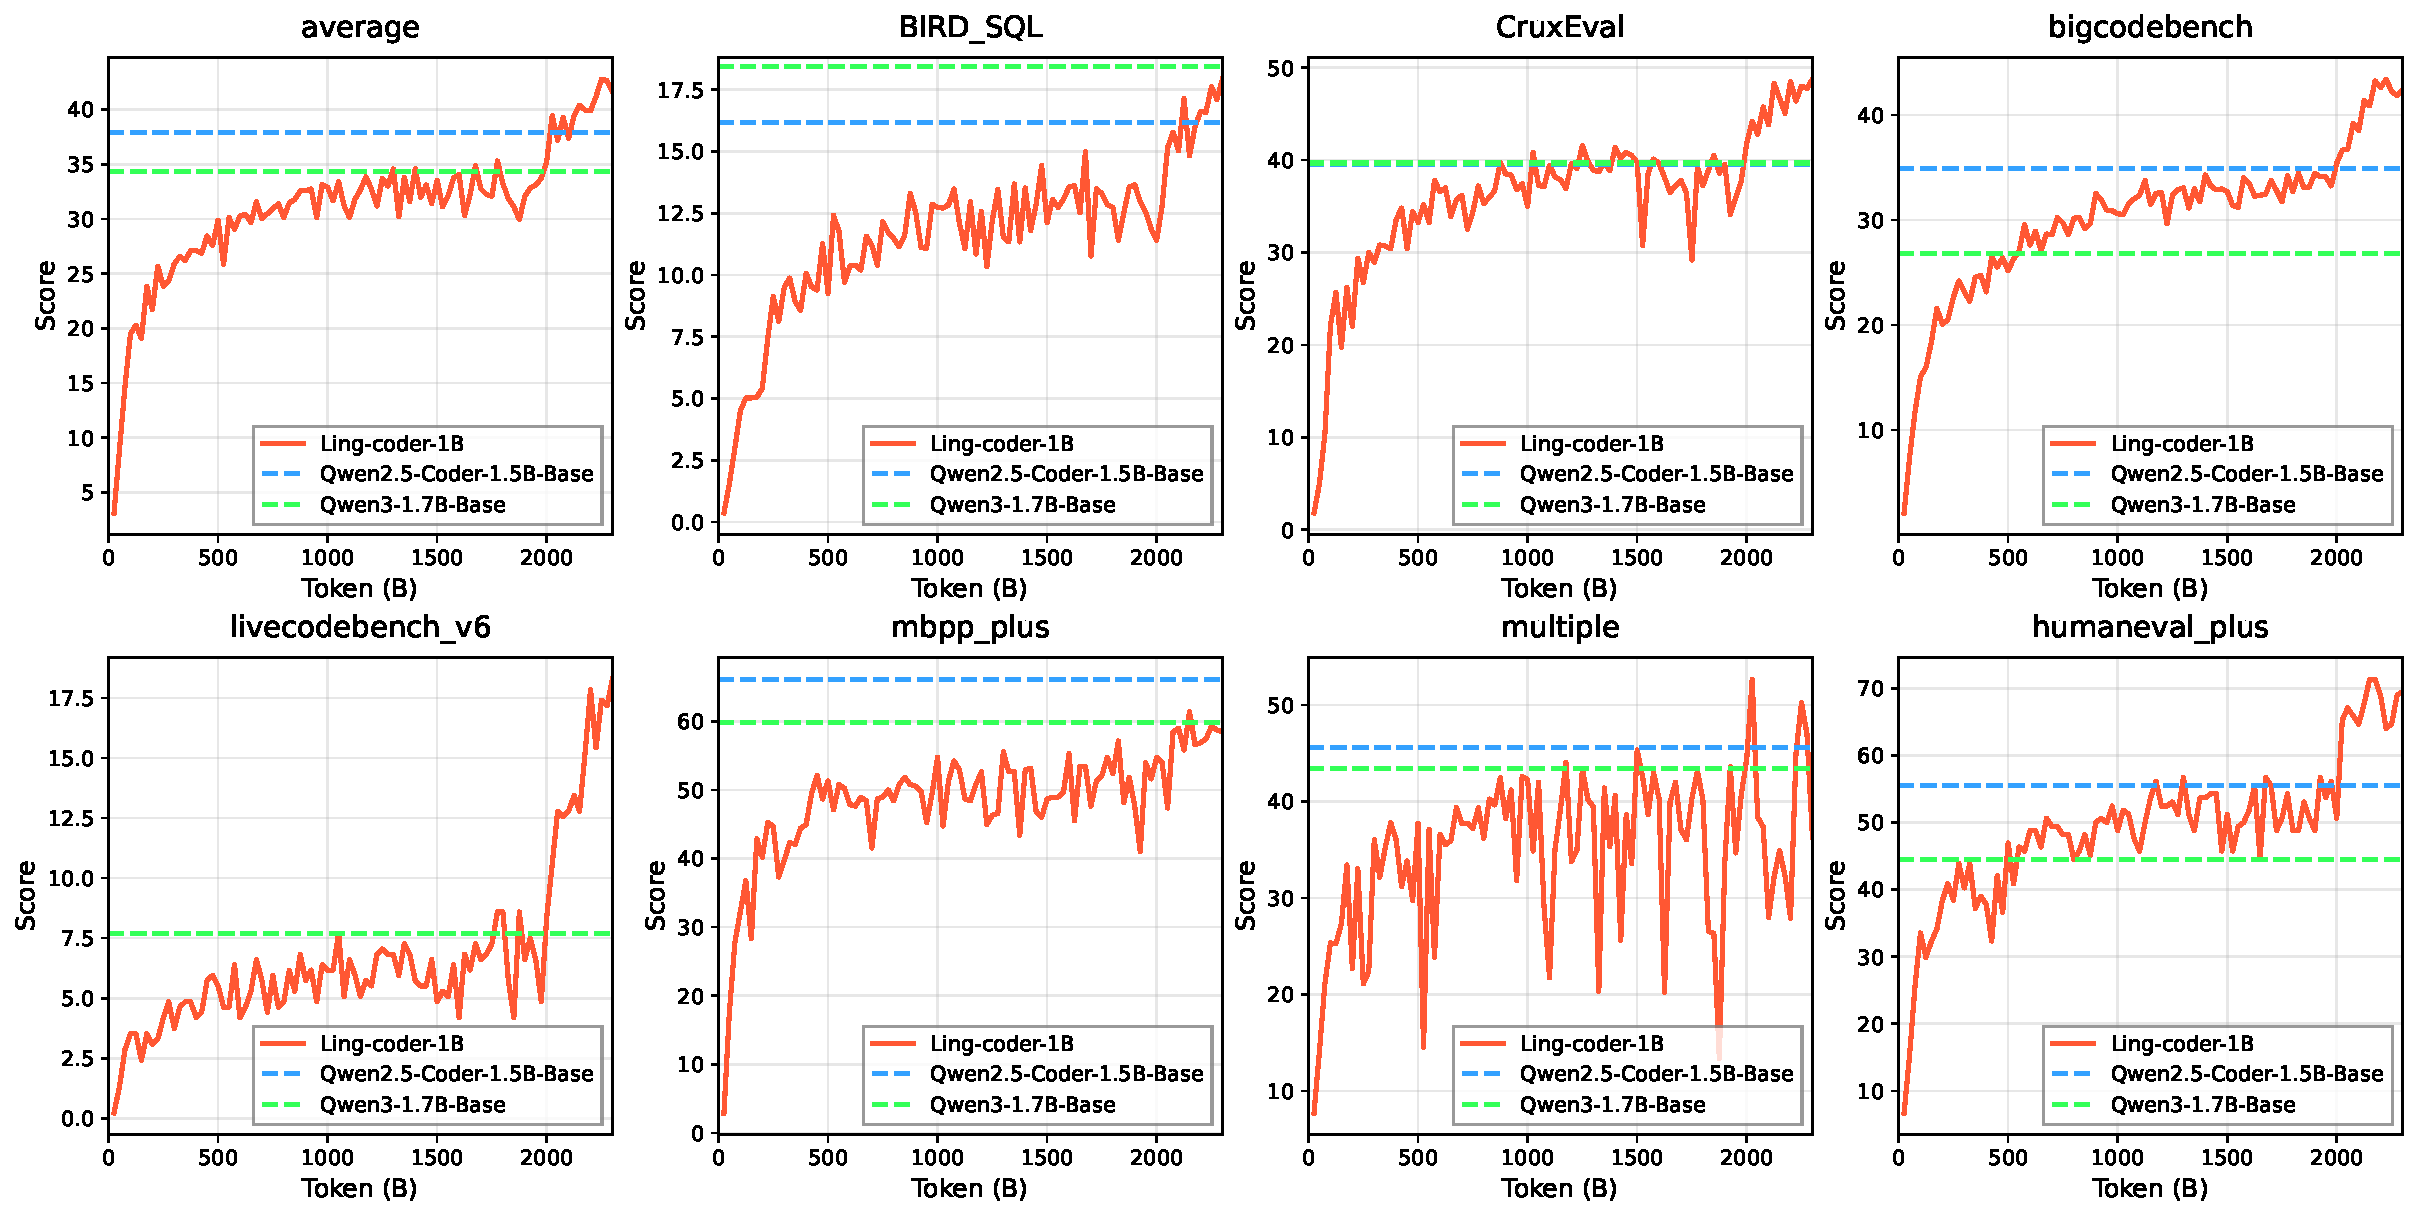
\includegraphics[scale=0.3]{figs/ling_math_coder.pdf}
    \caption{Experimental results to show the detailed performance of complete code corpus with 1B models.}
    \label{fig:coder-1b}
\end{figure}

\subsubsection{Ling Math Corpus}\label{appendix:math}
The mathematical proficiency of language models hinges on high-quality, diverse corpora. To train Ling 2.0 models of varying scales, we assembled a mathematics corpus exceeding 1.8T tokens, drawn from web pages, textbooks, research papers, code repositories, problem banks, and synthetic sources. A multi-stage processing pipeline—comprising parsing, recall, filtering, rewriting, and synthesis—was designed to curate this corpus. After careful balancing, the refined data constitutes the final pre-training mixture for our models.

{\bfseries General Math Data. }
Prior to construction of \emph{Ling Math Corpus}, we iteratively improved the PDF and HTML parser to ensure the completeness of mathematical content. After that, we develop a multi-stage pipeline to recall highly relevant math data from diverse sources including the web (e.g. Common Crawl), book, paper, and source code. First of all, we iteratively build a fastText classifier with a high recall ratio to locate math data inside a much smaller candidate pool. Next, we fine-tune small language models to develop LLM-Filter and LLM-Refiner with 4B parameters to filter out and refine data that contain mathematical knowledge or a step-by-step problem solving process. Upon applying the recall pipeline to diverse data sources along with employing deduplication technologies (e.g. MD5, MinHash), we collect a substantial volume of mathematical data comprising of web, book, paper \emph{etc}.

{\bfseries Synthetic Math Data. }
In addition, we employ synthetic data generation to create a diverse range of mathematical question-answer (Q\&A) pairs, varying in difficulty and incorporating step-by-step reasoning processes. This is performed on a high-quality recalled corpus sourced from multiple reputable origins. In parallel, we actively extract existing Q\&A pairs from web and book corpora. Furthermore, we synthesize entirely new math problems from scratch using a large-scale mathematical concept graph~\citep{chen2025arrows}, which contains thousands of nodes and millions of edges. This approach significantly expands the knowledge boundaries of our model. To complement this, we have also developed a sophisticated question generator designed to pose higher-quality and more realistic mathematical problems to the model.

{\bfseries Evaluating the Ling Math Corpus. }
To empirically validate the efficacy of our mathematical corpus, we use a continual-training then annealing strategy with only math corpus on a pre-trained Ling-coder-1B model introduced in Section \ref{appendix:coder} for over 1.8T tokens, in which the last 300B is used for annealing training. Due to the space limit, we only present the performance results on the average value of benchmarks. As shown in Figure~\ref{fig:math:a}, the resulting Ling-math-1B model exhibited performance superior to the competitive Qwen2.5-Math-1.5B-Base~\citep{yang2024qwen25mathtechnicalreportmathematical} and Qwen3-1.7B-Base~\citep{qwen3} on mainstream mathematical benchmarks (e.g. GSM8K~\citep{gsm8k}, MATH~\citep{math}, CollegeMath~\citep{college-math}, OlympiadBench~\citep{olympiadbench}, CMATH~\citep{cmath}, MathBench~\citep{mathbench} \emph{etc.}). This outcome substantiates the high quality of the integrated corpus.

Furthermore, a specific comparative analysis was conducted to evaluate the contribution of our curated mathematical web data. Using the same 1B-model training paradigm, we benchmarked our proprietary web data against a suite of well-regarded open-source datasets, namely Infi-mm-math~\citep{han2024infimmwebmath40badvancingmultimodalpretraining}, finemath-3plus~\citep{allal2025smollm2smolgoesbig}, megamath~\citep{zhou2025megamath}, and nemotron-cc~\citep{mahabadi2025nemotron}. The Ling-math-web-1B model trained on our web data demonstrated a markedly superior performance shown in figure~\ref{fig:math:web}. This finding empirically validates the effectiveness of our specialized web data acquisition and refinement pipeline, which constitutes a critical factor in the overall strength of our pre-training data.
\begin{figure}[t!]
    \centering
    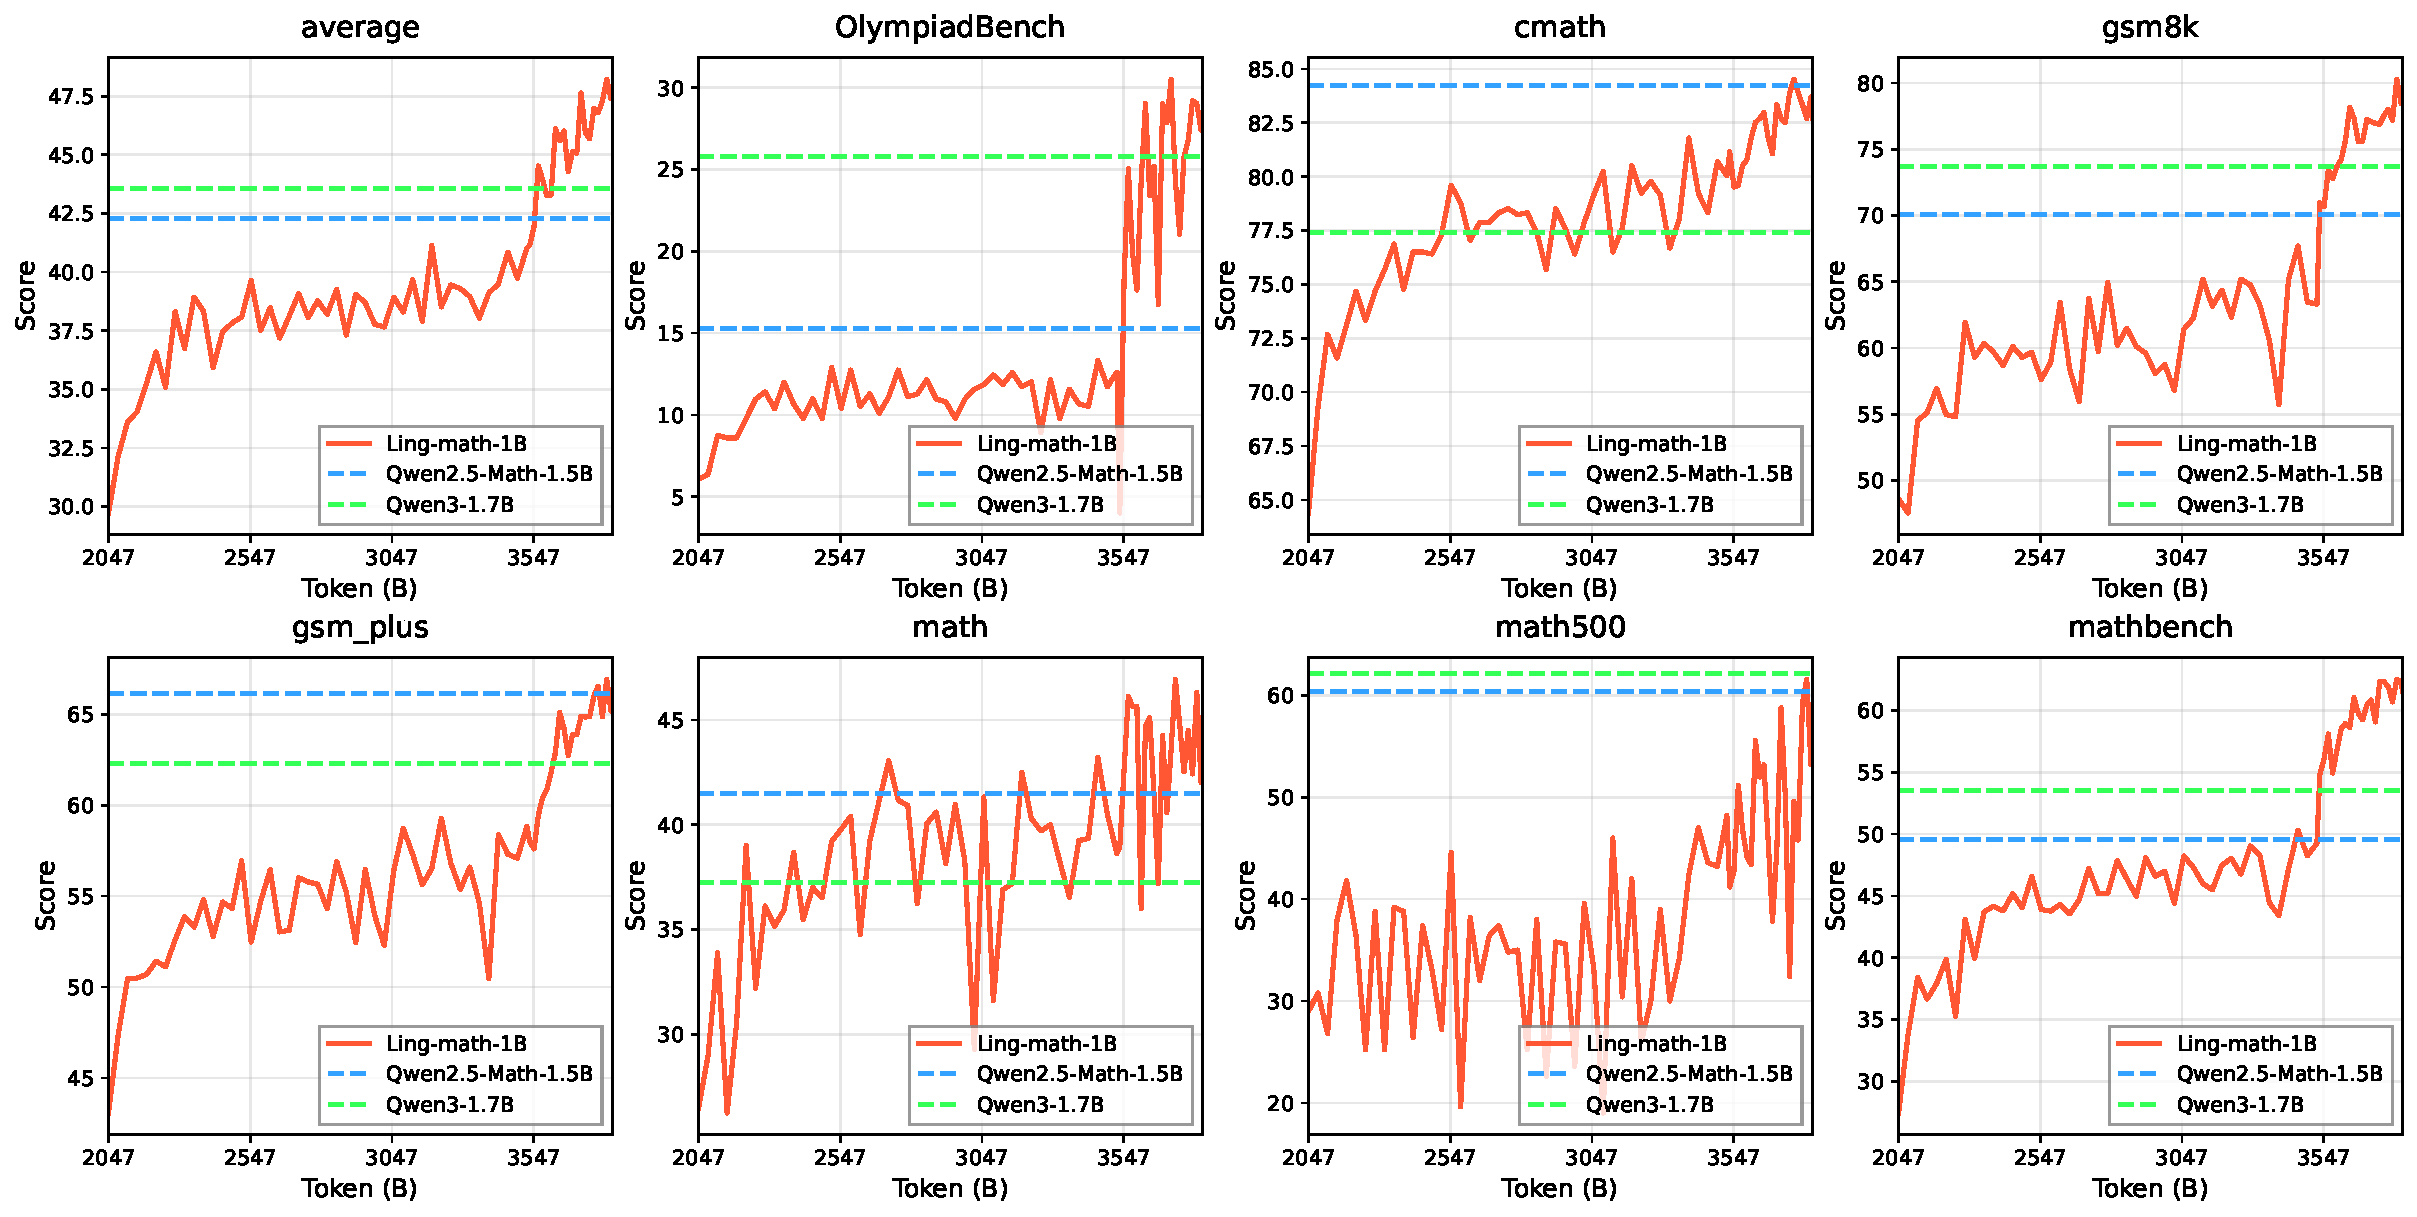
\includegraphics[scale=0.3]{figs/ling_math_1b_fig.pdf}
    \caption{Experimental results of LingMathCorpus on representative benchmarks.}
    \label{fig:math:complete}
\end{figure}

\begin{figure}[t!]
    \centering
    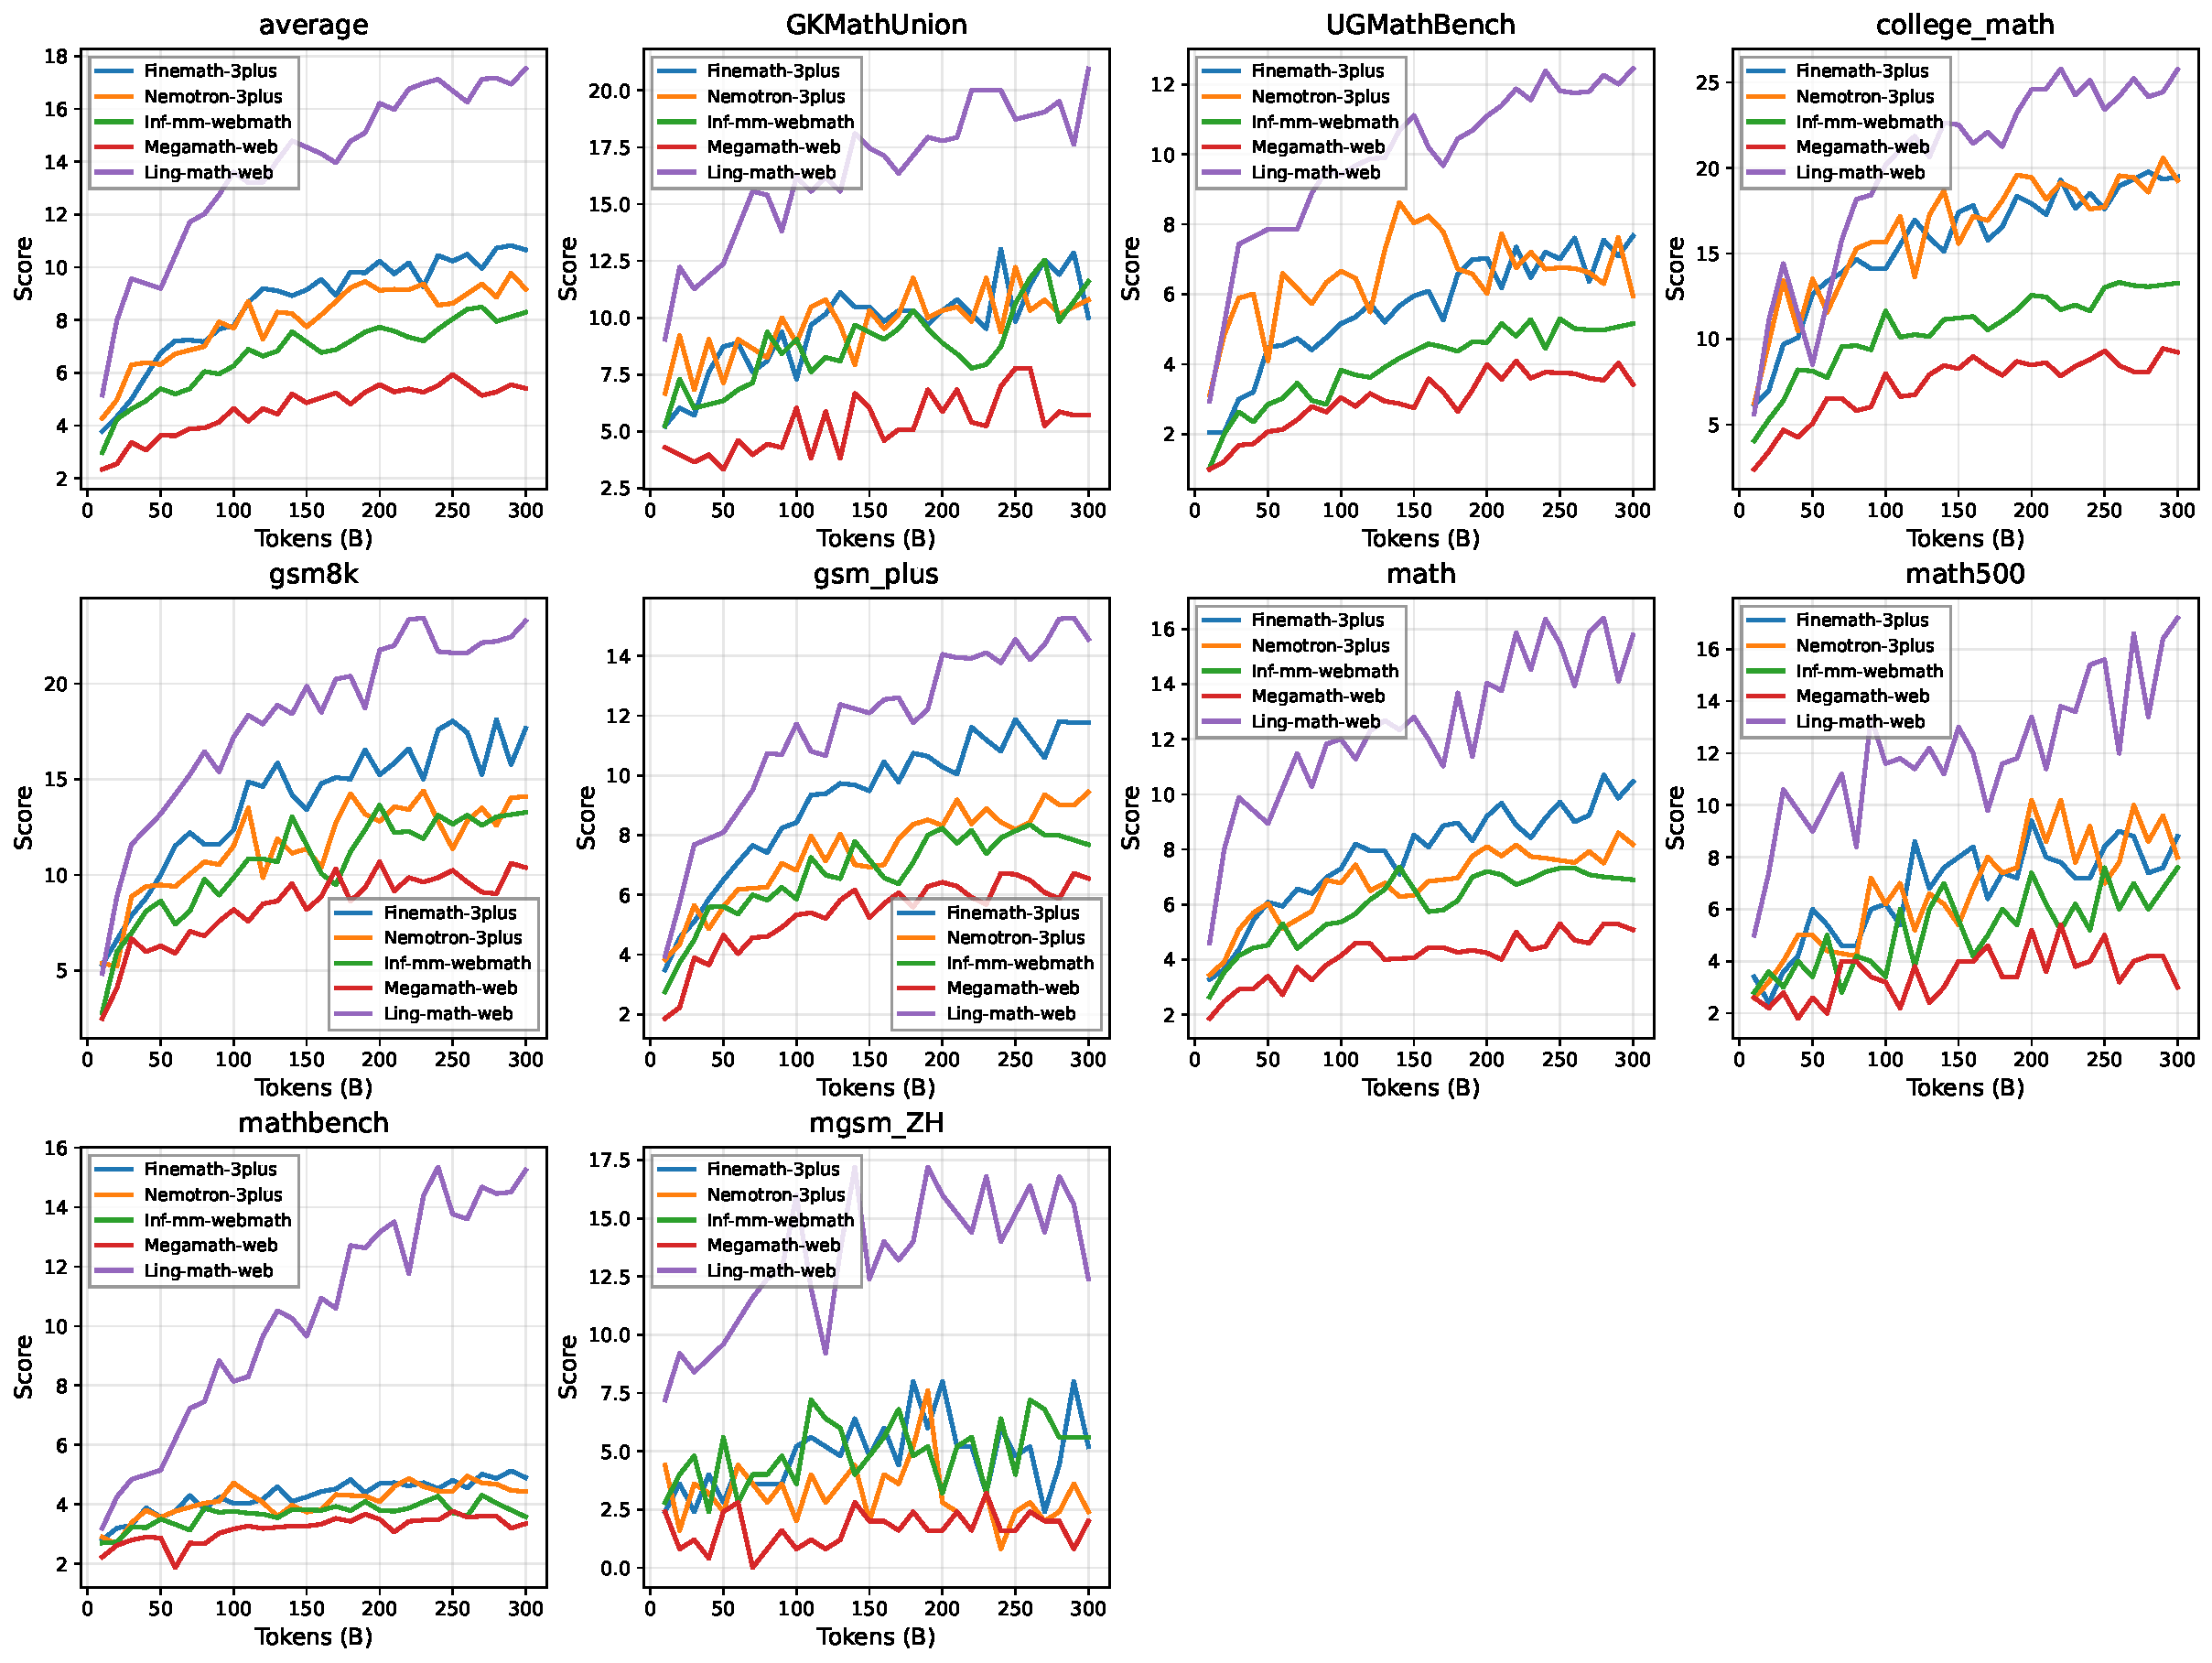
\includegraphics[scale=0.3]{figs/math_all_metrics.pdf}
    \caption{Complete comparison with open-source mathematical web data.}
    \label{fig:math:web}
\end{figure}


\subsection{Multilingual Data}
\label{sec:multilingual}
The 2TB of multilingual data is mainly from open-source web datasets, such as CulturaX \citep{multilingual_culturax} and WanJuan \citep{multilingual_wanjuan}, and we also involve several classical parallel corpora (OPUS \citep{multilingual_opus}, MultiUN~\citep{multilingual_multiun} \emph{etc.}) to strengthen the cross-lingual alignment. 

In terms of language distribution, our multilingual corpus covers about 30 languages in different domains such as web pages, code, mathematics, Wikipedia, parallel corpora, and a small amount of synthetic translation data. We first specifically include data from 18 individual languages, among which are
\begin{itemize}
    \item Germanic languages: German, Dutch, Swedish, Norwegian, Danish.
    \item Romance languages: Spanish, Portuguese, French, Italian, Romanian.
    \item Slavic languages: Russian, Polish, Ukrainian, Czech.
    \item Others: Vietnamese, Thai, Korean, Indonesian.
\end{itemize}

Furthermore, some corpora contain a mix of other languages, such as Japanese, Arabic, Hindi, Turkish, Finnish, \emph{etc.} are also used. 

Multilingual data accounts for 4\% of the pre-training corpus. The proportion by language family is about: Romance languages 50\%, Germanic languages 10\%, Slavic languages 3\%, and other languages the rest. The experiments find that this distribution maintains performance in Chinese and English, while significantly improving performance for minor languages. Data from Romance and Germanic languages have less negative effect on English and Chinese benchmarks, whereas lower-quality data from Slavic and other languages, especially Arabic or Japanese, can have a considerable negative effect. 

\subsection{Data Infrastructure}\label{appendix:data:infra}
Training large-scale language models poses significant challenges to the efficiency, scalability, and governance of data infrastructure. To address the pain points of traditional workflows, such as inefficient collaboration, opaque lineage, and slow iteration, we built a next-generation data infrastructure based on two core principles: \emph{Data-as-Code} and a \emph{Unified Data Lakehouse}.

{\bfseries Data-as-Code: From Manual Operations to Automated CI / CD. }
Our first principle is to codify the entire data processing pipeline and manage it within a version control system (e.g., Git) to achieve an automated and reproducible workflow. This methodology aligns with the design principles of the leading industry ML platforms, which aim to standardize and modulize the workflows for data processing and model training, managing them through code-driven orchestration~\citep{datainfra1}. Therefore, we developed a unified library for better managing \underline{AI} \underline{D}ata \underline{Op}erators (\emph{AIDataOps}), which centralizes over 50 data processing operators across multiple modalities, and integrated it into our automated CI/CD system. This transformation yields significant benefits: First, it provides an an end-to-end transparent and reproducible data lineage, making the origin of any data point clearly traceable. Second, it fully automates the development and backfilling of new features, dramatically increasing R\&D agility by reducing the iteration cycle from months to days.

{\bfseries Unified Data Lakehouse and Wide-Table Architecture. }
The second principle is the implementation of a unified lakehouse architecture to consolidate disparate data sources~\citep{datainfra2}. One of the biggest challenges for large-scale pretraining data management is that the data was scattered across hundreds of independent datasets, leading to severe data silos and inefficient experimentation. To solve this issue, we designed and implemented a unified logical wide table for major domains like web pages and code. This architecture acts as the central hub for all raw, processed, and trainable data. It not only simplifies data discovery and analysis through a unified view but also features elastic scalability, allowing new features to be added without full-table rebuilds. The system has been deeply optimized for large-scale training, achieving high-performance I/O of over 20 TB/hour and ensuring data processing is no longer a bottleneck.

By combining these two principles, we have created a powerful and efficient data engine. This infrastructure was instrumental in building the Ling 2.0 corpus. For instance, it enabled us to construct a wide table for all web data with trillions of records and to process 30 billion trainable data points in just two days. This system not only accelerates our current model development but also provides a solid foundation for more complex data exploration in the future.
